\documentclass{article}
\usepackage[backend=biber,citestyle=ieee]{biblatex}
\usepackage[english]{babel}
% \usepackage[swedish]{babel}
\usepackage{graphicx}
\usepackage{csquotes}
\usepackage{float}
\usepackage{datetime}
\usepackage[title]{appendix}
% \usepackage{a4wide} %For wider content on page
% \usepackage{amsmath} %For multiline equations 

\usepackage{fancyhdr}   %page header
\pagestyle{fancy}

% \usepackage[parfill]{parskip} %Line skip between paragraphs instead of indent

\usepackage{xcolor}
\usepackage{listings}

\definecolor{codegreen}{rgb}{0,0.6,0}
\definecolor{codegray}{rgb}{0.5,0.5,0.5}
\definecolor{codepurple}{rgb}{0.58,0,0.82}
\definecolor{backcolour}{rgb}{0.95,0.95,0.95}
\lstdefinestyle{mystyle}{
    backgroundcolor=\color{backcolour},   
    commentstyle=\color{codegreen},
    keywordstyle=\color{magenta},
    numberstyle=\tiny\color{codegray},
    stringstyle=\color{codepurple},
    basicstyle=\ttfamily\footnotesize,
    breakatwhitespace=false,         
    breaklines=true,                 
    captionpos=b,                    
    keepspaces=false,                 
    numbers=left,                    
    numbersep=5pt,                  
    showspaces=false,                
    showstringspaces=false,
    showtabs=false,                  
    tabsize=1
}
\lstset{style=mystyle}

\newcommand{\getauthor}{Elias Berglin} %Author
\newcommand{\gettitle}{Labb 1 - AR} %Title

\newdateformat{daymonthyear}{\ordinal{DAY} \monthname[\THEMONTH] \THEYEAR} %Date

\title{\gettitle}
\author{\getauthor}

\date{\daymonthyear\today} %Remove for swedish date

\begin{document}

    % Title 
    \pagenumbering{gobble}
    \maketitle
    \newpage

    % Page header and footer
    \pagenumbering{arabic}
    \fancyhf{}
    \lhead{\getauthor}
    \rhead{\gettitle}
    \rfoot \thepage

    % Document starts here
    \section{Week 1}
    \subsection{Assignment}
    \subsubsection*{1)  Derived a camera’s field of view $\theta$ as a function of focal length $f$ and sensor width $w$}
    From figure \ref{fig:focal} we can derive a function for $\theta$ as a function depending on $\alpha$ and we get the following equation:
    \begin{equation}
    \label{eq:startingEQ}
            \theta = 2\alpha
    \end{equation}
    \begin{figure}[H]
        \centering
        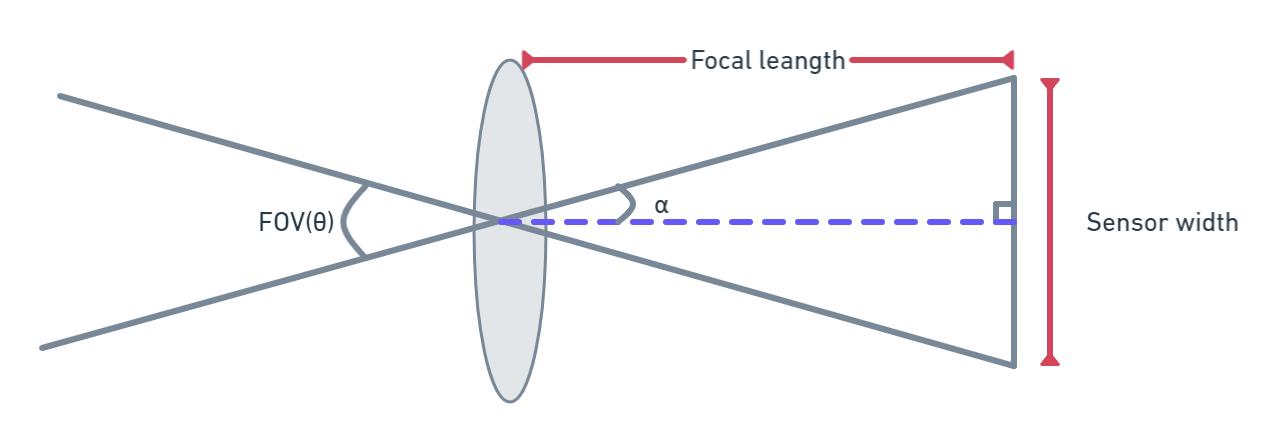
\includegraphics[width=1\textwidth]{focalLeanght.png}
        \caption{An illustration for deriving the formula for calculating field of view}
        \label{fig:focal}
    \end{figure}
    
    With equation \ref{eq:startingEQ} we can see that we need to find an expression for $\alpha$. From figure x we can derive $\alpha$ from the right angle triangle and with simple trigonometry we get the following formula:
    \begin{equation}
    \label{eq:AlphaStart}
        \frac{w}{2*f} = tan(\alpha)
    \end{equation}
    With equation \ref{eq:AlphaStart} we can now transform it to make it an expression of $\alpha$. This resuls in the following equation:
    \begin{equation}
    \label{eq:AlphaFree}
        \alpha = tan^{-1}\left(\frac{w}{2*f}\right)
    \end{equation}
    Now we can finally get an expression for $\theta$ with the help of equation \ref{eq:AlphaFree} and equation \ref{eq:startingEQ}. We get the following equation:
    \begin{equation}
    \label{eq:finalThetaEQ}
        \theta = 2*tan^{-1}\left(\frac{w}{2*f}\right)
    \end{equation}
    Equation \ref{eq:finalThetaEQ} shows the derived formula for calculating the field of view ($\theta$) as function of the focal length ($f$) and sensor width ($w$).
    \subsubsection*{2)  Allow two different cameras with sensor with $w_1$ and $w_2$ to have the same focal length $f$. Plot field of view $\theta_1$ and $\theta_2$ in a single graph.}
    The plot for $\theta$ as a function of $f$ for the sensor widths $w_1$ and $w_2$ is shown in figure \ref{fig:plot}.
    \begin{figure}[H]
        \centering
        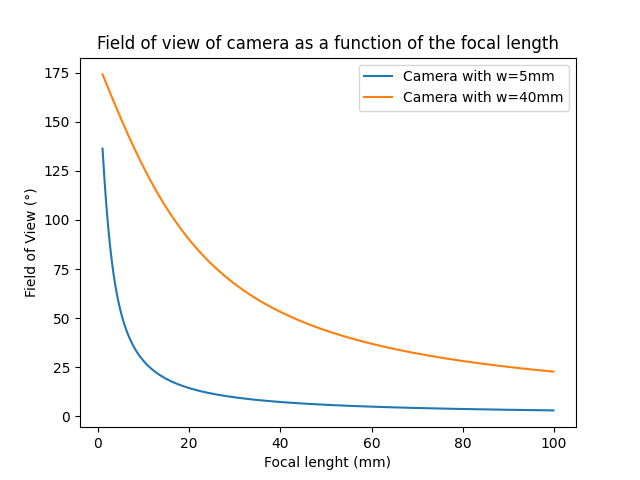
\includegraphics[width=1\textwidth]{Q2.png}
        \caption{Field of view as a function of focal length plotted with sensor width 5mm and 40mm}
        \label{fig:plot}
    \end{figure}
    \subsubsection*{3)  Consider two world points $x_1$ and $x_2$ and their projected 2D points $x_1^\prime$ and $x_2^\prime$ on the sensor plane. Let the points $x_1$ and $x_2$ be located in world space such that $x_1=(x, y, z)$ and $x_2=(x+dx, y, z)$. Evaluate how the distance between the projected points  $|x_2^\prime - x_1^\prime|$ varies as a function of focal lengths $f$ and depth $z$}
    Given focal length $f$ and coordinates $(x, y, z)$ we can calculate a projected 2D point with the formula from equation \ref{eq:projectionFormula}.
    \begin{equation}
        \label{eq:projectionFormula}
        \left( f\frac{x}{z}, f\frac{y}{z} \right)
    \end{equation}
    Since the only differentiating factor between $x_1$ and $x_2$ is the coordinate $x$ we can focus on that part and simplify the equation to:
    \begin{equation}
        \label{eq:SimplifiedProjectionFormula}
        |x_2^\prime - x_1^\prime| = \left| f\frac{x+dx}{z} - f\frac{x}{z} \right|
    \end{equation}
    Simplifying the expression from equation \ref{eq:SimplifiedProjectionFormula} we get the following:
    \begin{equation}
        \label{eq:finalProjection}
        |x_2^\prime - x_1^\prime| = \left| f\frac{dx}{z} \right|
    \end{equation}
    Equation \ref{eq:finalProjection} shows the final formula for calculating the distance between $x_1$ and $x_2$.
    \subsection{Reflections}
    The first week was stressful with the SIMS course overlapping. 
    I skipped reading the book and looked at the YouTube course. 
    The YouTube course provided a good explanation on the part of the assignment that was a bit unclear. 
    More specifically it provided good insight on the theory behind the third question and was helpful since lecture 1 overlapped to lecture 2. 
    The seminar at the end of the week cleared up the structure of the course. 
    The one weird thing I noticed is that there is not ethical discussion in the YouTube course, 
    I think that this should be an important part of any computer vision course. 
    The most interesting technique that I learned about this week was depth recovery from normal images.
    \section{Week 2}
    \subsection{Assignment}
    The Python code can be found in Appendix \ref{appendix:1}
    \subsection{Reflections}
    This week was a little better. 
    It was good to use the seminar to catch up on the rest of the lecture. 
    The assignment was interesting. 
    I simplified the assignment a bit and used cv2 to pad the image instead of padding it myself. 
    This week I got a bit more out of the seminar when I asked about the different color scales. 
    This week I had time to read the chapters in the book and watch the YouTube course. 
    In my opinion, the book is a bit all over the place. 
    Figures are placed a few pages back from where they were first referenced. 
    This made following the book harder. 
    The YouTube course is easier to follow, 
    and it cleared up some things I did not completely understand from the book.
    The most interesting for me this week was the different padding options when applying a kernel to keep the same size.  
    It was interesting to see how different padding techniques affected the image.

\newpage
    \begin{appendices}
        \section{Python code for image filter}
        \label{appendix:1}
        \begin{lstlisting}[language=Python]
            from matplotlib import image
    import numpy as np
    from matplotlib.image import imread
    from matplotlib.image import imsave
    from PIL import Image
    from numpy.core.fromnumeric import shape
    import cv2
    from skimage.exposure import rescale_intensity
    from skimage.exposure.exposure import _output_dtype
    
    
    def convolve(img, kernel):
        iH, iW = img.shape[:2]
        _, kW = kernel.shape[:2]
        pad = (kW - 1) // 2
        img = cv2.copyMakeBorder(img, pad, pad, pad, pad, cv2.BORDER_REPLICATE)
        output = np.zeros((iH, iW), dtype="float32")
    
        for y in np.arange(pad, iH + pad):
            for x in np.arange(pad, iW + pad):
                roi = img[y - pad:y + pad + 1, x - pad:x + pad + 1]
                k = (roi * kernel).sum()
                output[y - pad, x - pad] = k
        output = rescale_intensity(output, in_range=(0, 255))
    
        output = (output * 255).astype("uint8")
        return output
    
    
    def convolveRGB(img, kernel):
        iH, iW = img.shape[:2]
        _, kW = kernel.shape[:2]
        pad = (kW - 1) // 2
        img = cv2.copyMakeBorder(img, pad, pad, pad, pad, cv2.BORDER_REPLICATE)
        output = np.zeros((iH, iW, 3), dtype="float32")
    
        for y in np.arange(pad, iH + pad):
            for x in np.arange(pad, iW + pad):
                roi = img[y - pad:y + pad + 1, x - pad:x + pad + 1]
                r = (roi[:, :, 0] * kernel).sum()
                g = (roi[:, :, 1] * kernel).sum()
                b = (roi[:, :, 2] * kernel).sum()
                k = [r, g, b]
                output[y - pad, x - pad] = k
        output = rescale_intensity(output, in_range=(0, 255))
    
        output = (output * 255).astype("uint8")
        return output
    
    
    roi = np.array(([
        [[250, 253, 251], [250, 253, 251], [250, 253, 251]],
        [[250, 253, 251], [250, 253, 251], [250, 253, 251]],
        [[250, 253, 251], [250, 253, 251], [250, 253, 251]]
    ]), dtype="int")
    
    
    sharp = np.array((
        [0, -1, 0],
        [-1, 5, -1],
        [0, -1, 0]), dtype="int")
    
    blurr = np.array(([
        [0.0625, 0.125, 0.0625],
        [0.125, 0.25, 0.125],
        [0.0625, 0.125, 0.0625]]), dtype=float)
    
    edge = np.array(([
        [-1, -1, -1],
        [-1, 8, -1],
        [-1, -1, -1]
    ]), dtype="int")
    
    rightSobel = np.array(([
        [-1, 0, 1],
        [-2, 0, 2],
        [-1, 0, 1]
    ]), dtype="int")
    
    emboss = np.array(([
        [-2, 1, 0],
        [-1, 1, 1],
        [0, 1, 2]
    ]), dtype="int")
    
    gblurr = np.array(([
        [1, 4, 6, 4, 1],
        [4, 16, 24, 16, 4],
        [6, 24, 36, 24, 6],
        [1, 4, 6, 4, 1],
        [4, 16, 24, 16, 4]
    ]), dtype="float")
    
    gblurr = gblurr * (1/256)
    
    umask = np.array(([
        [1, 4, 6, 4, 1],
        [4, 16, 24, 16, 4],
        [6, 24, -476, 24, 6],
        [1, 4, 6, 4, 1],
        [4, 16, 24, 16, 4]
    ]), dtype="float")
    
    umask = umask * (-1/256)
    
    img = cv2.imread("bilder/ill.png")
    img = cv2.cvtColor(img, cv2.COLOR_BGR2RGB)
    
    save = Image.fromarray(img)
    save.save('original.png')
    
    
    print("Sharpening")
    sharpend = convolveRGB(img, sharp)
    save = Image.fromarray(sharpend)
    save.save('sharp.png')
    
    print("Blurring")
    blurred = convolveRGB(img, blurr)
    save = Image.fromarray(blurred)
    save.save('blurr.png')
    
    print("Detecting edges")
    edged = convolveRGB(img, edge)
    save = Image.fromarray(edged)
    save.save('edge.png')
    
    print("Right sobel")
    rSobel = convolveRGB(img, rightSobel)
    save = Image.fromarray(rSobel)
    save.save('right_sobel.png')
    
    print("Emboss")
    em = convolveRGB(img, emboss)
    save = Image.fromarray(em)
    save.save('embossed.png')
    
    print("G-blurr")
    gb = convolveRGB(img, gblurr)
    save = Image.fromarray(gb)
    save.save('gblurr.png')
    
    print("umask")
    um = convolveRGB(img, umask)
    save = Image.fromarray(um)
    save.save('umask.png')
    
        \end{lstlisting}
    \end{appendices}
\end{document}